\chapter{Introduction}
\addcontentsline{toc}{chapter}{Introduction}
%
\linenumbers
%
Modern society faces a wide range of challenges that require complex and multifaceted solutions. The challenges posed by climate change and the necessity for clean energy in order to reduce greenhouse gas emissions intersect with the goals of economic growth and the global exchange of information, goods and people. Unprecedented issues are emerging from this increasingly technologically advanced and interconnected civilization. 

This PhD work was initiated amidst the most impactful public health crisis of our time, the COVID-19 pandemic. Despite all the negative facets of this pandemic, it unexpectedly gave a boost to a specific market : the emerging technology of deep ultraviolet violet light-emitting diodes (UVC LEDs), and the market is predicted to grow five-fold.\cite{Yole} Indeed the deep UV light, \textit{i.e.} with wavelengths ranging from 100 to 280 nm, has been demonstrated to inactivate the coronavirus accountable for the disease, thus making it harmless.\cite{GERCHMAN2020112044} Besides surface disinfection, UVC LEDs have many applications in water and air depolution, agriculture, printing and more.\cite{hsu2021perspectives} The material studied in this thesis, hexagonal Boron Nitride, is a candidate of choice for the elaboration of UVC LEDs due to its bright light emission in the deep ultraviolet.

This is a recent example of how technological innovations resulting from scientific research in materials science can provide a means to address the challenges of modern society. The European Union supports such research in particular through the Flagship projects, which are large-scale research initiatives with an emphasis on technology transfer to industry. Three out of the four Flagship projects are closely related to materials science : Batteries30+ for the development of efficient and compact energy storage,\cite{batteries_flagship} Quantum Technologies\cite{quantum_flagship} for the quantum computers and algorithms and Graphene,\cite{graphene_flagship} which focuses on two-dimensional materials. All of these are research projects that could provide means to produce clean energy and store it. In all of these scientific areas, theory and numerical simulations are essential to support the experimental discovery of materials and guide the engineering of new devices. This is particularly relevant in Condensed Matter Physics which is the subject of this thesis. Since the discovery of Graphene and its extraordinary properties by Novoselov and Geim,\cite{novoselov2004electric} the two-dimensional (2D) materials such as Graphene, black Phosphorus, transition metal dicalchogenides (TMDs) and hexagonal Boron Nitride (hBN) have attracted much attention. Indeed, they exhibit a range of electronic and optical properties that allow the design of devices for different applications, especially when different layers are stacked to form the so-called van der Waals heterostructures.\cite{geim2013van} The resulting devices are then very compact and fit very well into the technological trend of device miniaturization.

With the variety of optical and electronic properties offered by all the existing monolayers, and the ability to engineer them with factors such as stacking of different layers,\cite{sponza2018direct} twisting angle between them,\cite{latil2023structural, impellizzeri2022electronic} and straining\cite{blundo2021strain} as well as their interaction with substrates, the possibilities for devices are almost limitless. In this ecosystem, hexagonal Boron Nitride is a candidate of choice for its structural, electronic and optical properties.

% 


\section{Explain luminescence}
%
%					
%		 CORRECT THIS
%
%
%
Optical measurements are an efficient way to characterize materials and reveal the microscopic, quantum, interplay between electronic wavefunctions and electromagnetic field of light, and collective quantum effects in the crystal.\cite{dressel2002electrodynamics} In particular, spontaneous emission of light after an excitation, known as \textit{luminescence}, is the key property for the elaboration of light-emitting diodes. 

For spontaneous light emission to happen in a semiconductor or insulator, there needs to be excited electrons populating the conduction band. The excitation can have different forms. It can be done with the electromagnetic field of external light, then the process is called photoluminescence. If the electrons are excited by an external beam of electrons colliding with the crystal, it is called cathodoluminescence. If they are excited by an external electric field, it is called electroluminescence, \textit{et cetera}. When the electrons are promoted to the higher-energy conduction bands, they leave an empty state in the valence band. This empty state can be thought of as a \textit{hole} in the Fermi sea of the valence states. It propagates with the opposite of the electron's momentum and has a negative effective mass. For light to be emitted, the excited electrons need to de-excite and go back to the empty states. We speak of radiative recombination of an electron-hole pair. When the hole and the electron have the same momentum (and the same spin and symmetry) the radiative recombination can happen because the emitted light carries an almost zero momentum, hence respecting momentum conservation. The energy difference between the electron and the hole corresponds to the frequency of emitted light, multiplied by $\hbar$. 
However when the bottom of the conduction band is not at the same momentum than the top of the valence band, the light emission cannot happen directly because of momentum conservation. There needs to be a second-order process to exchange momentum. The excited electron can transfer its momentum to another one and then recombine with the hole. This process is known as Auger-Meitner recombination.\cite{delaney2009auger} Otherwise, the momentum exchange can come from the absorbtion or emission of a phonon, hence gaining or losing energy and momentum and finally leading to a radiative recombination. This is known as a phonon-assisted transition and it is the process that is studied in this thesis. 

Luminescence is often thought of as the reverse process of light absorption. Indeed in absorption, light with a frequency higher than the gap can excite electrons and promote them to the conduction band, with almost zero transfer of momentum. In the case of phonon-assisted transitions, the electron can be promoted to the conduction band at another momentum, thanks to the absorption or emission of a phonon. 

Because of this similarity, the spectra of absorption and of luminescence are quasi symmetrical for direct transitions. The asymmetry come from the phonon broadening of the electron density of states, known as the Stokes shift. However when considering phonon-assisted transitions, some negligible features of the optical absorption spectra become dominant in the luminescence ones. The spectra can look very different, as illustrated by the experimental results presented in Fig. \textcolor{red}{Figure}. For bulk hexagonal Boron Nitride, the state dominating the absorption is different from the one dominating the luminescence, which is at lower energy. Moreover, since the phonon-assisted transitions appear as multiple peaks, there is a strong asymmetry in the spectra. This will be explained in details in the body of this thesis.

In this thesis, we study the properties of different forms of hBN and develop theoretical and numerical methods with the aim of reproducing and predicting their luminescence spectra from \textit{ab initio} calculations.




%
%
%
%
\section*{Paragraph on the properties of hBN}
The first reported synthesis of Boron Nitride dates back from 1842.\cite{balmain1842xlvi} It is now available commercially under the form of a white powder and finds applications as lubricant and for its high thermal resistivity. It can be found under the form of a layered material composed of atomically thin layers arranged in a honeycomb lattice. High-purity crystals are synthesized under high-pressure and high-temperature conditions.\cite{watanabe2004direct} 
Different stacking of the layers lead to different stable or metastable polytypes. In this thesis we will be mainly concerned with the AA' and the AB stackings, that are illustrated in Fig. \ref{fig:hBN_stackings}. We will refer to the AA' polytype as hBN and to the AB polytype (or Bernal phase) as bBN. The atoms within a layer are bond by hybrid $sp^2$ bonds, while the interlayer interactions are of van der Waals type.
\begin{figure}[h!b]%
	\vspace{0.2cm}
	\setcapindent{2em}
	\centering
    \subfloat[AA' stacking]{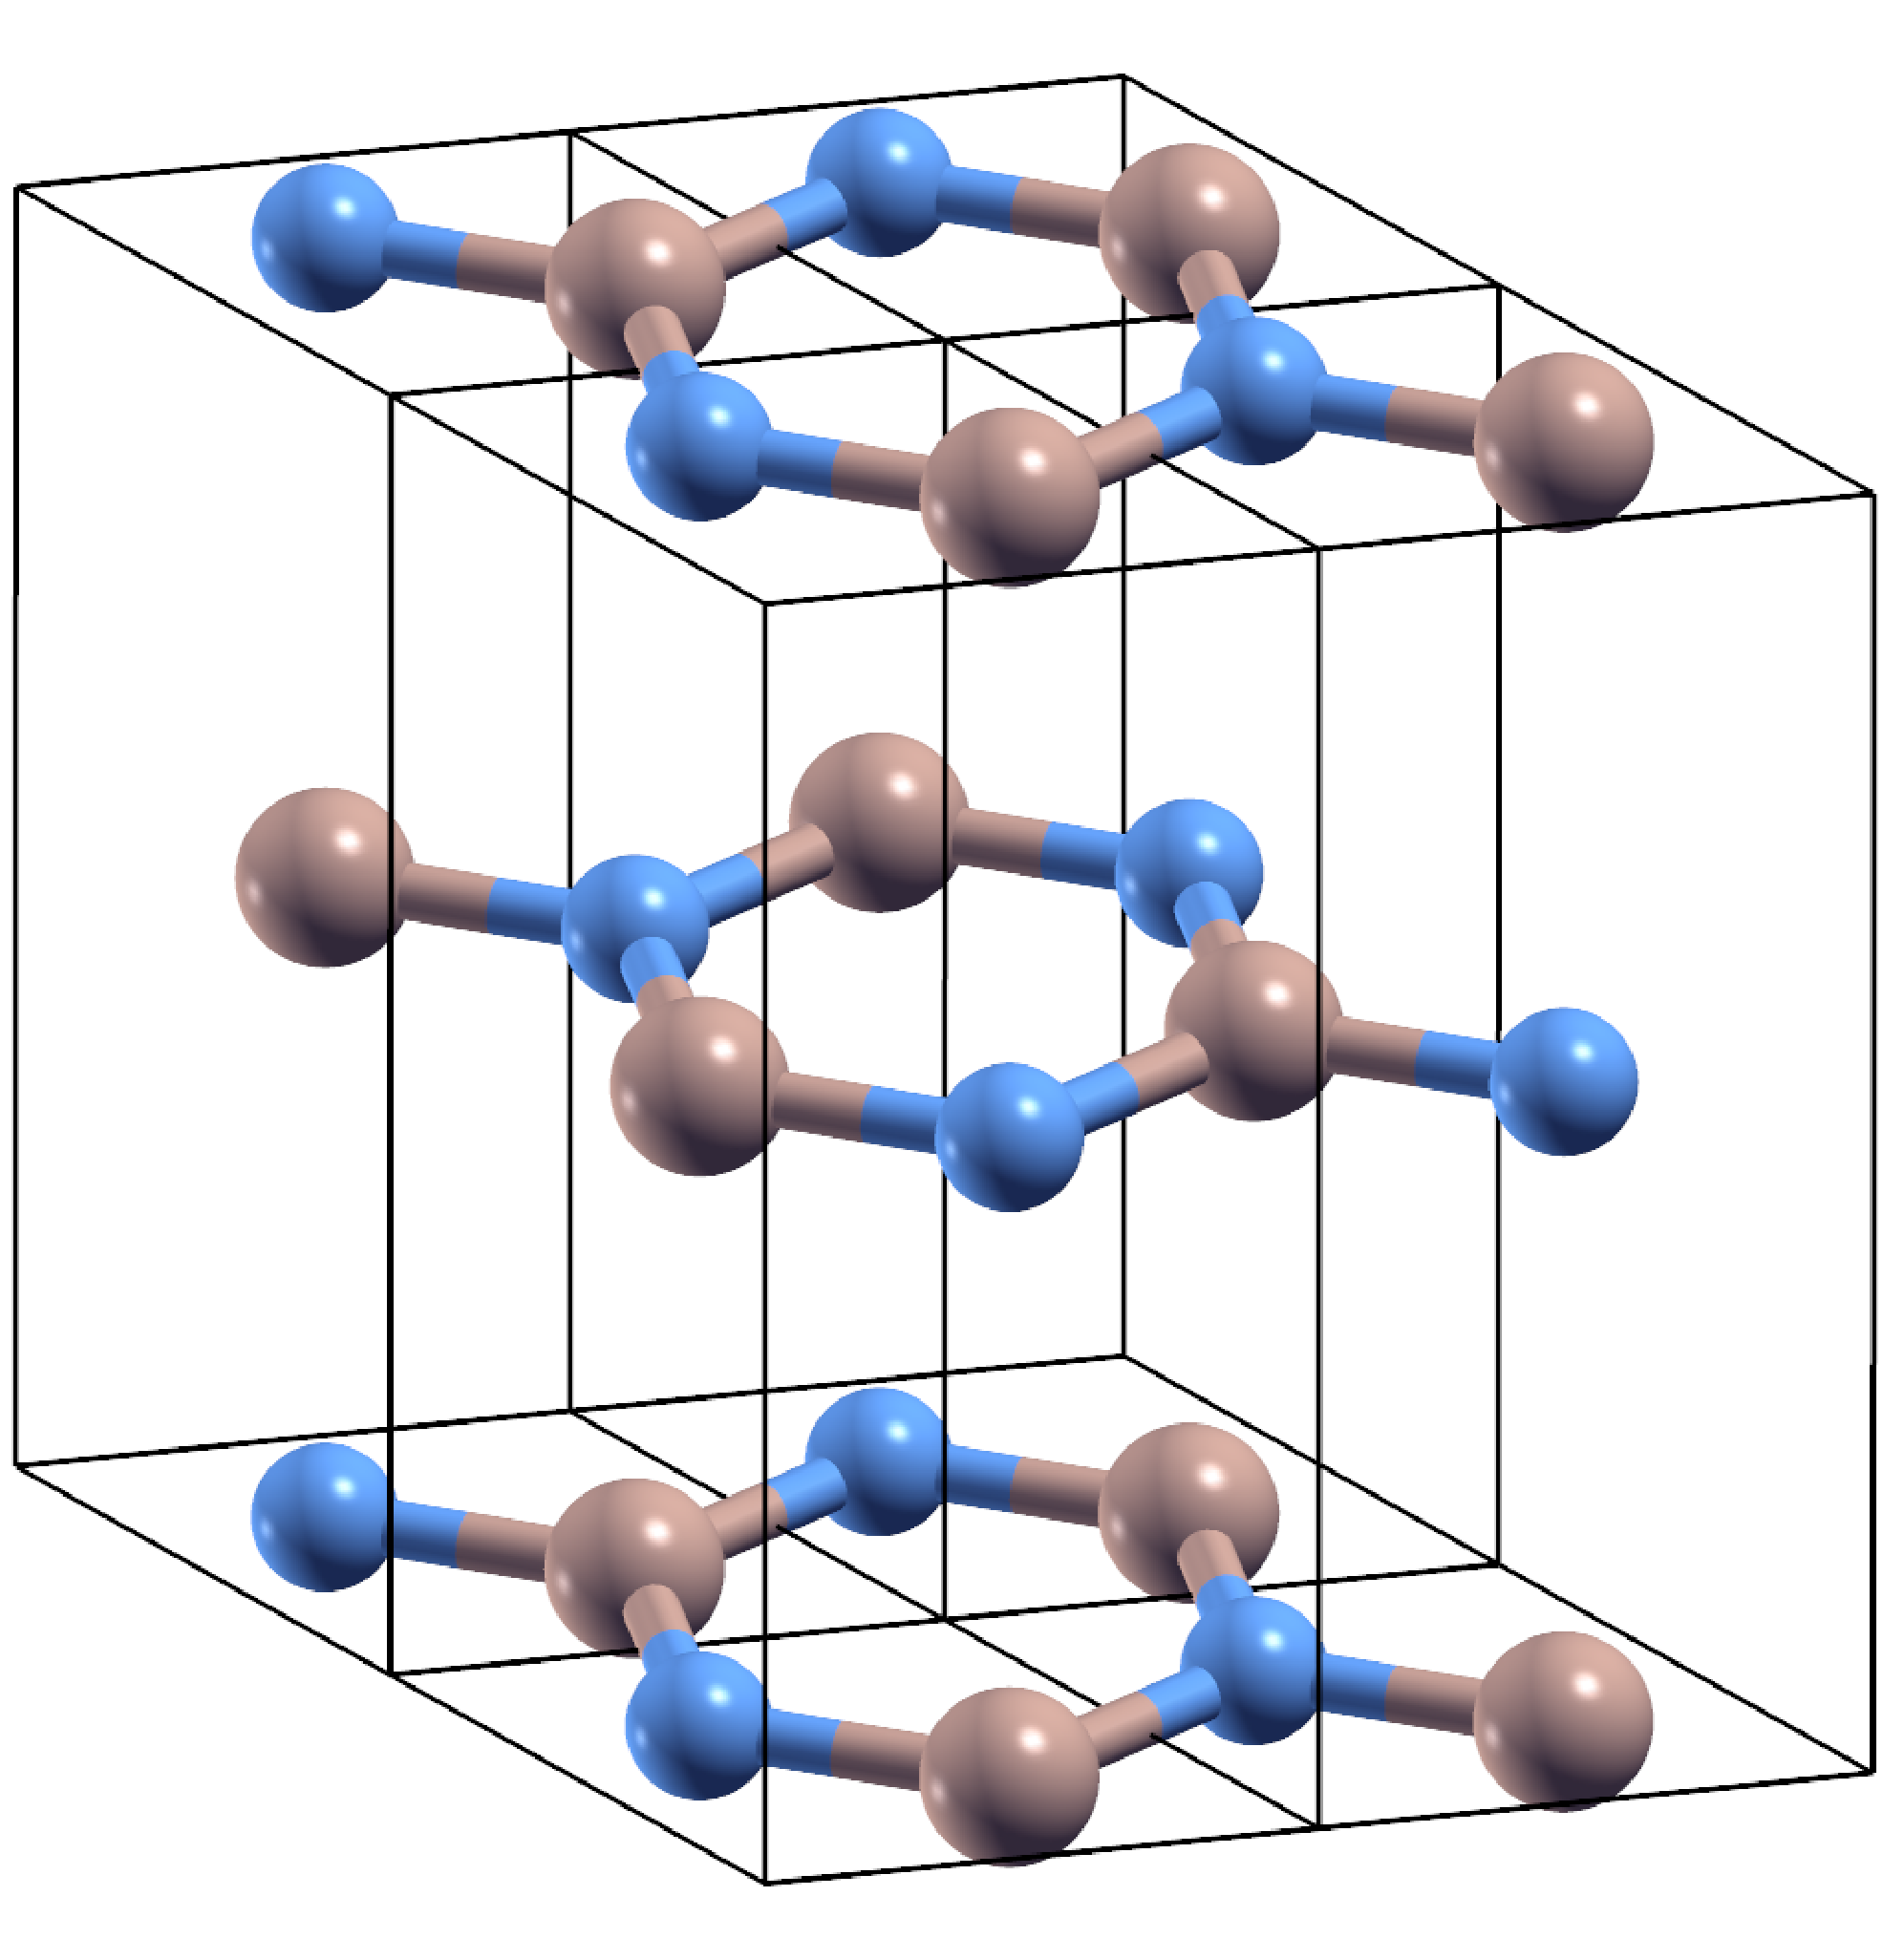
\includegraphics[width=0.42\textwidth]{intro/hBN_struc_crop.pdf}} \qquad
    \subfloat[AB stacking]{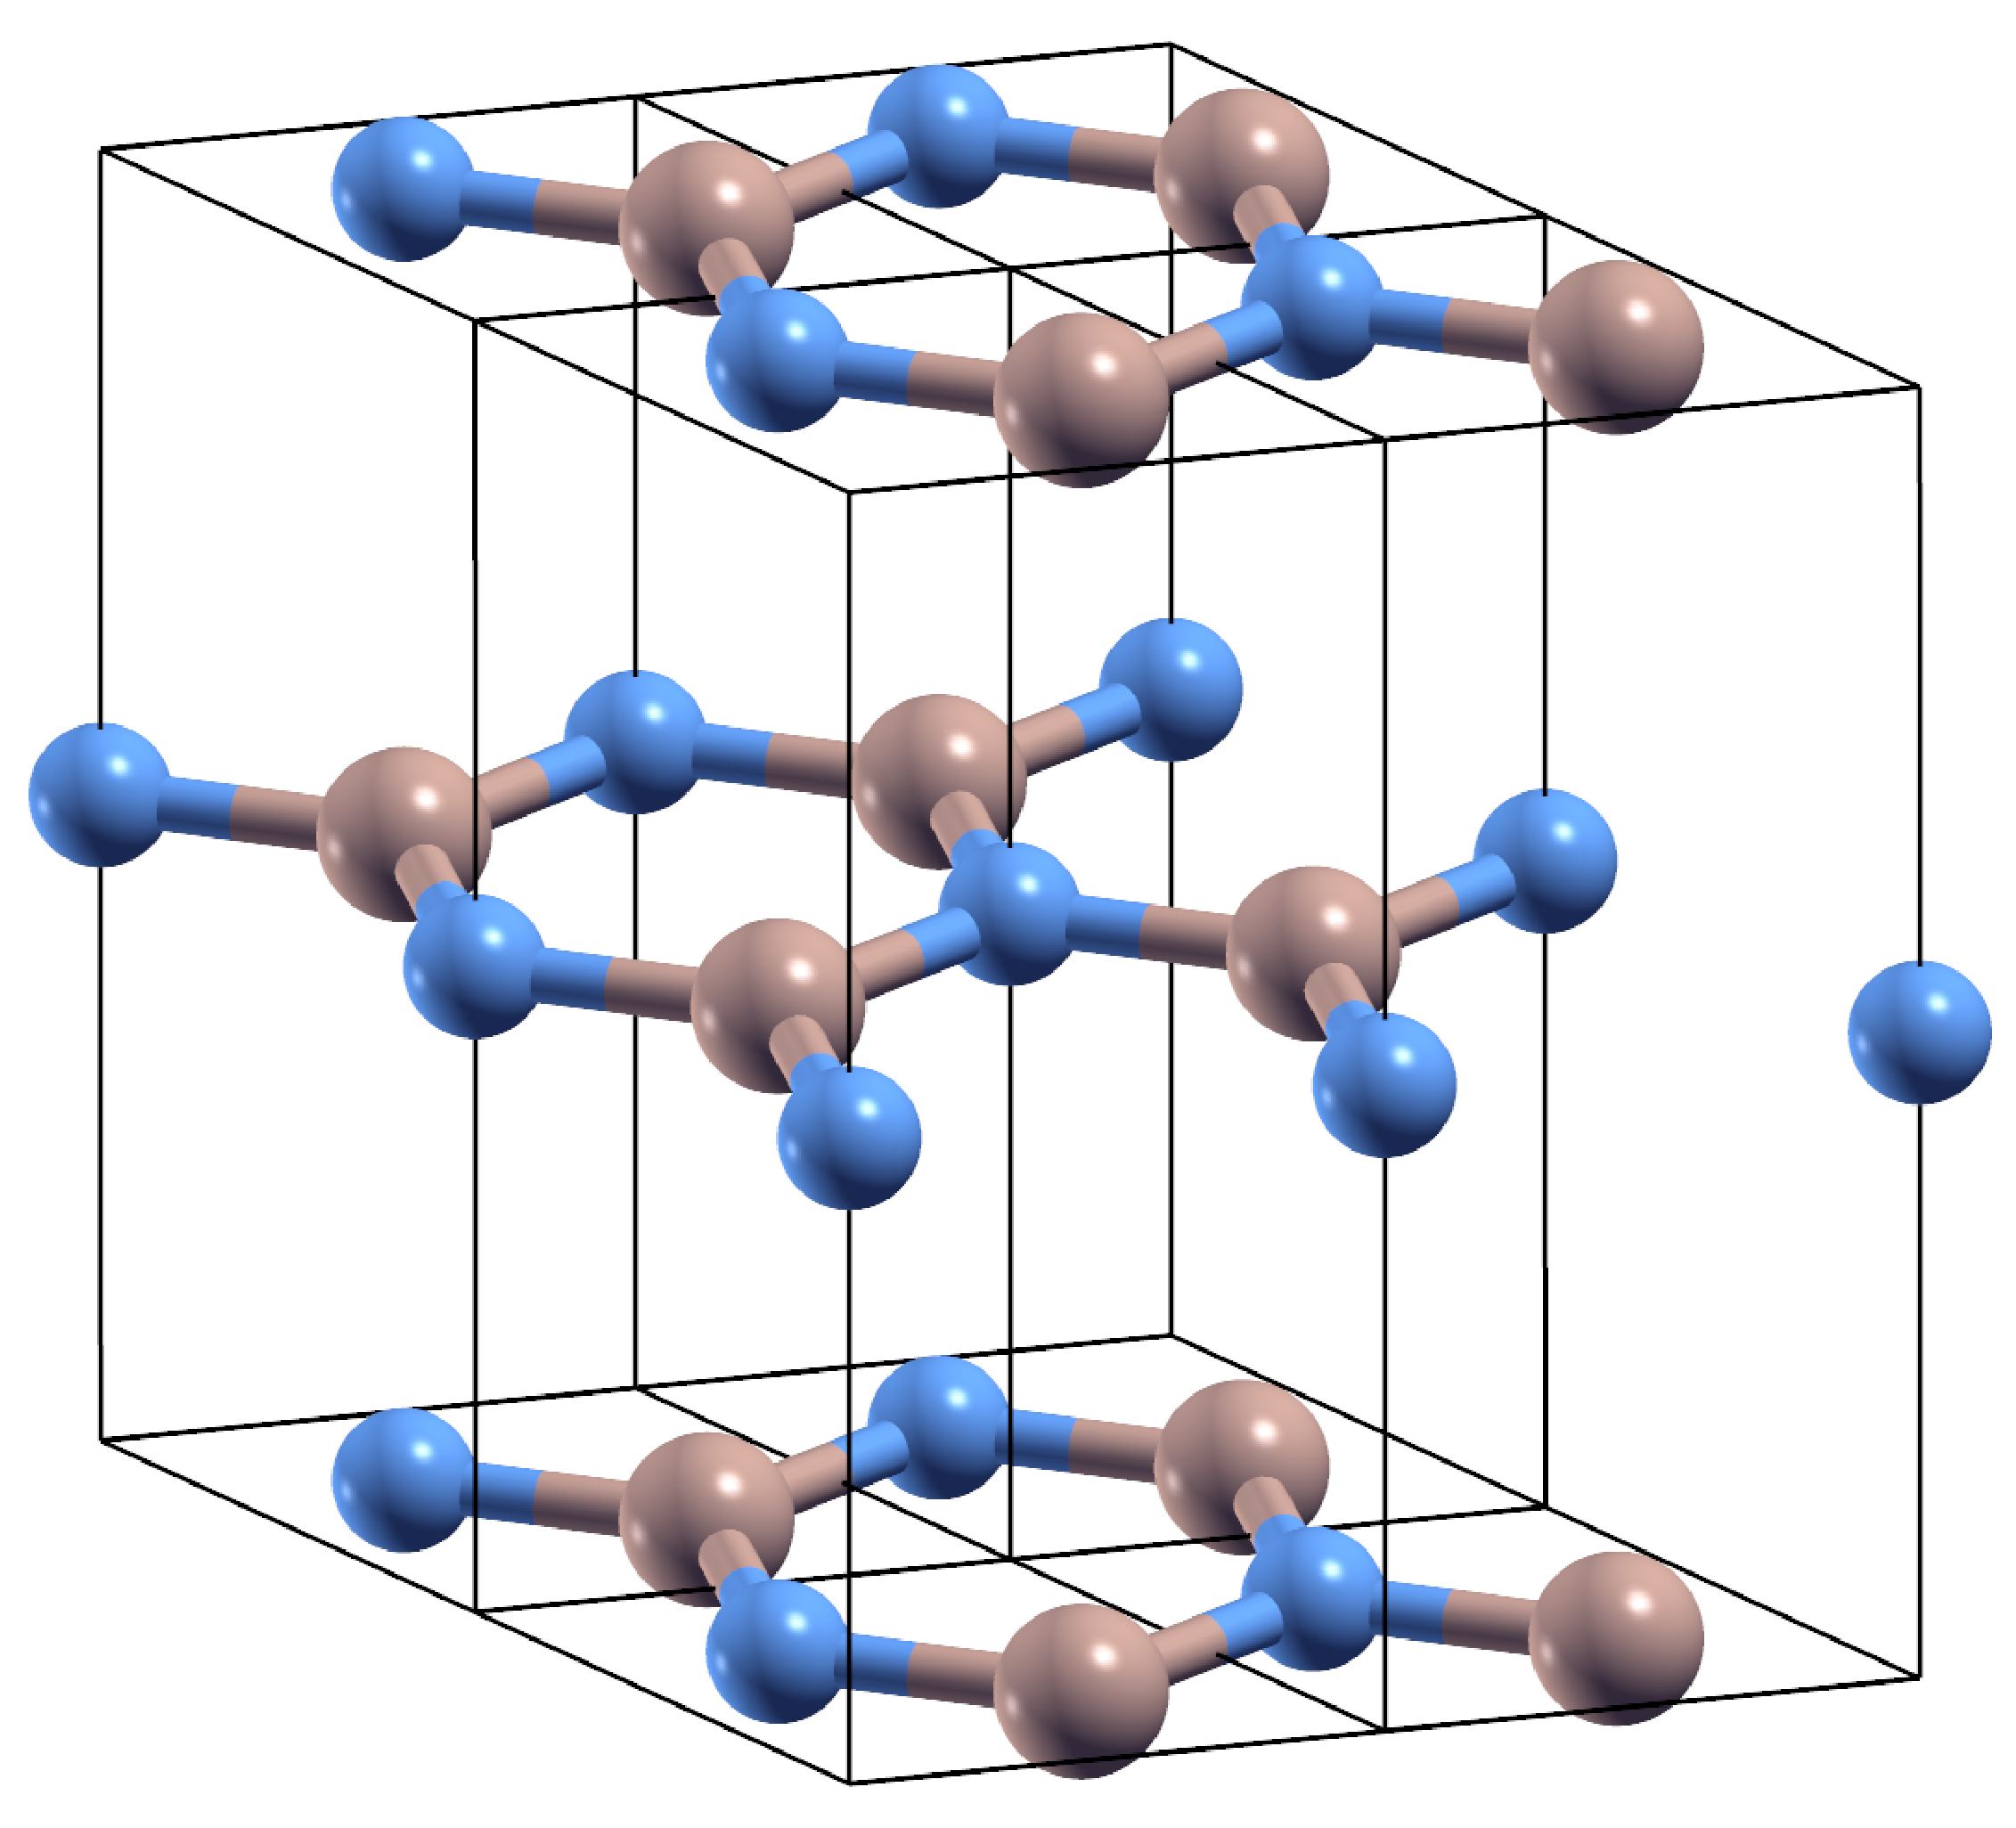
\includegraphics[width=0.45\textwidth]{intro/bBN_struc_crop.pdf}}%
    \caption{Two polytypes of hexagonal Boron Nitride where four hexagonal unit cells are shown. Boron atoms are represented with brown spheres, Nitrogen with blue ones. We will refer to the AA' polytype as hBN and to the AB polytype (or Bernal phase) as bBN.}
	\label{fig:hBN_stackings}
\end{figure}
%
hBN is stable at ambient pressure and room temperature. It is an insulator with a gap of about 6 eV. Due to its low lattice mismatch with Graphene and its insulating character, it is a substrate of choice and a good encapsulation layer for Graphene-based applications.\cite{kretinin2014electronic} It also has a variety of defect-related physics,  applications for quantum computing,\cite{ivady2020ab} single photon emission\cite{grosso2017tunable} or bright color center emission.\cite{wigger2019phonon} However the property of interest for this thesis is the bright light emission in the deep UV domain and the rich features appearing in the luminescence spectra. hBN was shown to have a very external quantum efficiency, comparable to that of a direct gap material such as Zinc Oxyde.\cite{schue2019bright} This is due to the strong exciton-phonon coupling enhanced by the anisotropy of this layered material. 
\textcolor{red}{ptite compil des spectres expérimentaux}
%
show electronic bands : hig gap, pDOS of valence at K is mostly Nitrogen, $\pi$ orbital(overlap of $p_z$, bonding)  . pDOS of conduction at M is mostly Boron, $\pi^*$ orbital \cite{galvani2016excitons,sponza2018direct}(overlap of $p_z$ with opposite coefficient, antibonding)\\


% Where to put this paragraph ?
Absorption is relatively easy to obtain from state-of-the-art \textit{ab initio} calculation, but luminescence is more difficult since it is an out-of-equilibrium process. For hBN it is the opposite on the experimental side of things : since the gap is very large, one needs high-frequency lasers for absorption, or synchrotron radiation as in Fig. \textcolor{red}{fig abs hBN}. Luminescence spectra are it less dependent on the excitation so its easier, but still we need low temperature to be able to resolve all the phonon peaks individually. When talking about a single layer it is even harder since the intensity of emitted light is low. This explains the very recent appearance of luminescence spectra of monolayer hBN in the scientific literature.

absorption 


Gorbachev, Roman V., et al. "Hunting for monolayer boron nitride: optical and Raman signatures." Small 7.4 (2011): 465-468.
% @article{gorbachev2011hunting,
%   title={Hunting for monolayer boron nitride: optical and Raman signatures},
%   author={Gorbachev, Roman V and Riaz, Ibtsam and Nair, Rahul R and Jalil, Rashid and Britnell, Liam and Belle, Branson D and Hill, Ernie W and Novoselov, Kostya S and Watanabe, Kenji and Taniguchi, Takashi and others},
%   journal={small},
%   volume={7},
%   number={4},
%   pages={465--468},
%   year={2011},
%   publisher={Wiley Online Library}
% }


Bernal :  C.-J.  Kim,  L.  Brown,  M.  W.  Graham,  R.  Hovden,  R.  W.Havener, P. L. McEuen, D. A. Muller, and J. Park,Nano Lett.13,5660(2013)
% @article{kim2013stacking,
%   title={Stacking order dependent second harmonic generation and topological defects in h-BN bilayers},
%   author={Kim, Cheol-Joo and Brown, Lola and Graham, Matt W and Hovden, Robert and Havener, Robin W and McEuen, Paul L and Muller, David A and Park, Jiwoong},
%   journal={Nano letters},
%   volume={13},
%   number={11},
%   pages={5660--5665},
%   year={2013},
%   publisher={ACS Publications}
% }


\begin{itemize}
	\item structure
	\item synthesis
	\item electronic bands and phonons (flat bands, HK transitions \cite{fugallo}
	%@article{elias2021flat,
% 	title={Flat bands and giant light-matter interaction in hexagonal boron nitride},
% 	author={Elias, Christine and Fugallo, Giorgia and Valvin, Pierre and L’Henoret, Christian and Li, J and Edgar, JH and Sottile, F and Lazzeri, M and Ouerghi, A and Gil, Bernard and others},
% 	journal={Physical Review Letters},
% 	volume={127},
% 	number={13},
% 	pages={137401},
% 	year={2021},
% 	publisher={APS}
%   }
  )
	\item paper with synchrotron absorption (big excitonic effects)
	\item PL spectra of bulk
	\item CL spectra of few layers, difficulty of PL for monolayer
	\item first experimental PL spectra of monolayer (say that we exploit them in Chap 3) 
\end{itemize}




\section{Scope of the thesis}
%
The state-of-the-art theoretical framework in which our calculations are contained starts from the adiabatic approximation.\cite{martin2020electronic} It states that the electronic and the atomic motions can be decoupled because of the mass difference between nuclei and electrons.

We then make use of the widely used \acrfull{DFT}.\cite{kohn1996density} In this theory the electrons are treated as independent particles evolving in a mean-field. It allows to compute the ground state density of the crystal and to obtain the equilibrium geometries, with a certain set of approximations. From there we extract the Kohn-Sham eigenvalues and wavefunctions. These eigenvalues give an approximation to the band structure and are the starting point of the more involved \acrfull{MBPT}. 

\acrshort{MBPT} is based on Green's functions and treats the many-body interactions as a perturbation of the independent-particle system. The main equations of this theory are the Hedin's equations.\cite{hedin1965new} Truncating this set of coupled self-consistent equations by neglecting the electron-hole interaction gives on one hand the \acrfull{RPA} to account for the dynamical electronic screening and on the other hand the \acrfull{GWA}. In the latter, the matrix product of the electronic propagator $G$ and the dynamically screened interaction $W$ gives the \textit{self-energy} $\Sigma$. It can be interpreted as a non-local, frequency-dependent potential that dresses the independent electrons with the interactions with other electrons, which is an improvement with respect to the mean-field of \acrshort{DFT}. The electrons become \textit{quasiparticles}, whose evolution in time and space is easier to describe than the full many-electrons system.
With this we are able to obtain a more accurate band structure and simulate experiments that involve charged excitations -- \textit{i.e.} addition or removal of an electron of the system. 

However the neutral excitations of the many-electron system -- \textit{i.e.} an electron being excited but staying in the system -- are not well described at this point. To this end, the electron-hole interaction is reintroduced by computing the two-particle Green's function. This is the solution of the so-called \acrfull{BSE}.\cite{blase2020bethe} Starting from the $GW$ approximation, the \acrshort{BSE} can be formulated in the basis of \textit{excitons}, which are quasiparticles made of an electron-hole pair, bound together by the Coulomb interaction. From the \acrshort{BSE} one can obtain the response function of the system including excitonic effects, with the assumption that excitations are instantaneous in time and response to these excitations. This is known as the \textit{static} approximation. Excitons have been shown to play a significant role in the optical spectra of \acrshort{hBN} and indeed the \acrshort{BSE} description is in much better agreement with experiments compared to independent-particles or quasiparticles levels of theory, as can be seen in Fig. \textcolor{red}{Figure of absorption}. A link can be made between microscopic excitonic quantities and macroscopic observables measured experimentally. 

Finally, we use a perturbative method based on \acrshort{DFT} to obtain the vibrational properties of the crystal in the harmonic approximation, meaning that each atom is represented as an harmonic oscillator vibrating around its equilibrium position. It is called \acrfull{DFPT}.\cite{baroni2001phonons} In second quantization, it gives a description of the vibrational modes of the lattice in terms of quanta of vibration called \textit{phonons}. They are another type of quasiparticle, that is a collective excitation, with a definite frequency and wave vector, analogous to the crystal momentum of electrons. We can now reintroduce the coupling between nuclear and electronic motions and formulate the electron-phonon coupling in second quantization. We obtain the coupling matrix elements that are the probability amplitudes that a electron is scattered by a phonon from a given momentum-energy state into another, where the energy and momentum is exchanged with the phonon.  


In condensed matter, the problem of exciton-phonon coupling and phonon-assisted luminescence is an old topic. The first studies date back to the 1960s by Toyozawa \emph{et al.}\cite{toyozawa2003optical,toyozawa1964interband} and the first dynamical solution of the \acrshort{BSE}, the so-called Shindo solution, was proposed precisely to study the exciton-phonon problem.\cite{shindo1970effective}
For model semiconductor quantum wells, the time-evolution of correlation functions, that includes simultaneous exciton-phonon and exciton-photon scattering, was studied in Ref. \cite{thranhardt2000quantum}. However this approach requires material-dependent parameters and is computationally expansive for real materials.

With the increase in computing capabilities, computationally heavy theories such as \acrshort{MBPT} became in reach and further developed to study more challenging materials. We can cite a few works on this regards such as the study of exciton-phonon coupling to the optical absorption of carbon nanotubes with combined tight-binding and \textit{ab initio} approach by Perebeinos \textit{et al.}.\cite{perebeinos2005effect}. There is also the theory of Hallen-Bardeen-Blatt for phonon-assisted absorption, \cite{hall1954infrared} applied in first-principles for Silicon,\cite{noffsinger2012phonon} an approach valid only for indirect semiconductors. 

Zacharias \textit{et al.} derived a formalism based on Williams-Lax theory\cite{williams1951theoretical,lax1952franck} to treat phonon-assisted transitions on the same footing as vibrational renormalization of the electronic band structures, but only for independent particles.\cite{zacharias2016one} They further included excitonic effects in the optical absorption from finite differences \cite{huang2021exciton} in monolayer Germanium Selenide. This methodology is based on a finite-difference derivative scheme to compute the exciton-phonon coupling. This goes beyond previous approaches developed independently by Paleari \textit{et al.} in Ref. \cite{paleari2019exciton} and Cannuccia \textit{et al.} in Ref. \cite{cannuccia2019theory} in the sense that in the two latter references, the renormalization of the exciton energies due to the coupling with phonon is neglected. It is well suited for the study of large indirect gap semiconductors and insulators and indeed they applied the methodology to the calculation of phonon-assisted luminescence of bulk hBN, which were the first times such spectra were obtained from first principles. This is the approach we will present in detail in Chapter \ref{chap:strain} and that we applied to the study of luminescence of strained hBN. 

However, in order to simulate any kind of gapped material, the dynamical renormalization of the direct emission peak intensity due to interaction with phonons needs to be considered. This way, one can obtain accurate spectra for materials that exhibit both direct exciton peaks and phonon-assisted replicas in their luminescence spectra. Such modern formulations in \acrshort{MBPT} can be mentioned, such as the polaron transformation in Ref. \cite{feldtmann2009phonon}, the use of the density matrix in Ref. \cite{brem2020phonon}, the formulation in terms of two-particle Green's functions from Ref. \cite{antonius2017theory} or the more general real-time approach from Ref. \cite{paleari2022exciton} as well as the cumulant \textit{ansatz} to include scattering of excitons with multiple phonons from Ref. \cite{cudazzo2020first}

The approach we present in Chapter \ref{chap:mBN} to compute the exciton-phonon matrix elements is the first order of the cumulant expansion of the latter reference. We obtain it by treating the interaction of excitons and phonons with second-order perturbation theory. This allows to obtain an exciton-phonon interaction Hamiltonian. We get exciton-phonon coupling matrix elements equivalent to those of Ref. \cite{chen2020exciton}, although we compute the luminescence in a different way, based on a steady-state approximation.
We can reformulate the Hamiltonian problem in the form of a response function including a dynamical correction due to scattering with phonons. This correction gives rise to the appearance of phonon-assisted peaks in the optical spectra, and it yields the renormalization of the direct excitonic peaks. The main advantage of this \textit{ab initio} approach is that we can compare the direct and indirect, phonon-assisted process in the luminescence spectra, while doing all the necessary calculations in the unit cell.

A sketch of the computational steps necessary to obtain the exciton-phonon coupling and phonon-assisted luminescence is drawn in Fig. \ref{fig:workflow}.
\begin{figure}[h!b]
	\vspace{0.2cm}
	\setcapindent{2em}
	\centering
	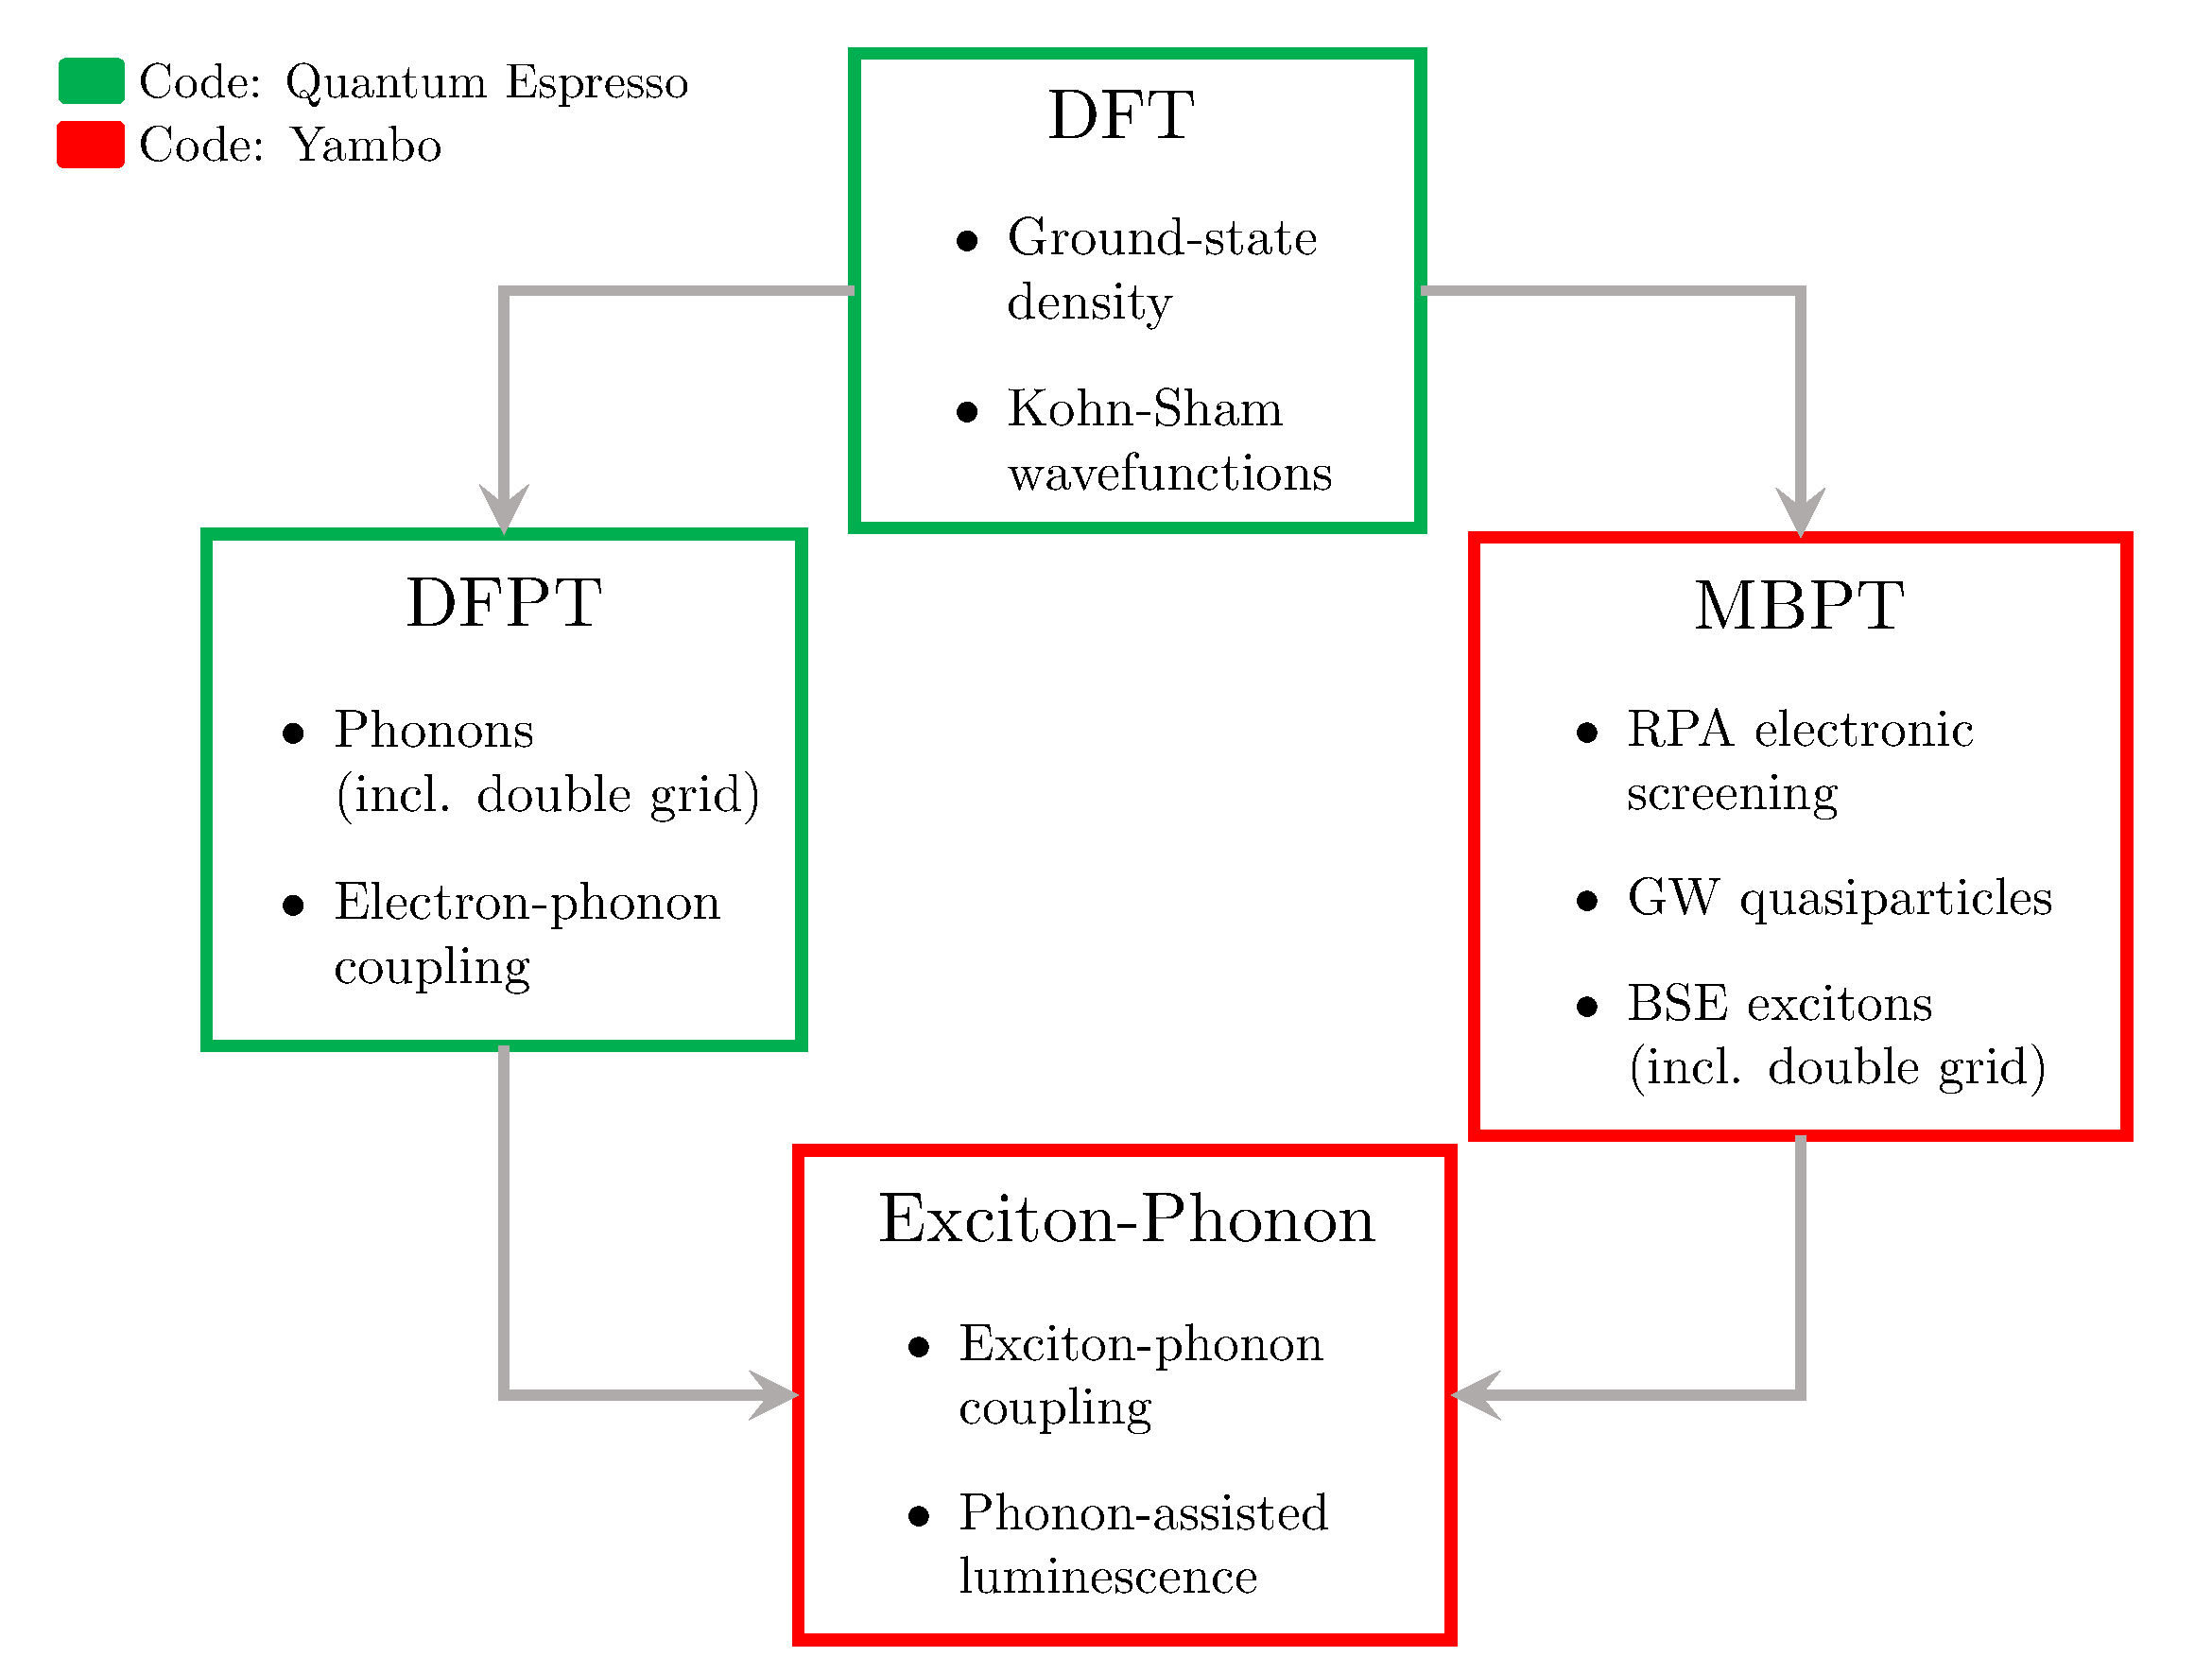
\includegraphics[width=0.9\textwidth]{intro/workflow_detailed.pdf}
	\caption{Workflow of the calculations to compute exciton-phonon coupling and phonon-assisted luminescence. The green and red boxes indicate that we used \textsc{Quantum ESPRESSO} and \yambo~as simulation codes, respectively.}
	\label{fig:workflow}
\end{figure}


\section{Structure}
This thesis is organized as follows : the 
Chap 2 , Hedin's equations whose derivation is sketched in this first Chapter.
describe chapter 3 strain
describe chapter 4 mBN
appendices


% ETSF webinar of Fulvio
% indirect bandgap only; we can write the response function with derivatives of the response function because we consider only phonon-assisted transitions; need supercells
% PLE (propto absorption) or absorption and PL are not symmetric, as expected for direct gaps
% the minimum exciton at T is the degenerate dark state at Gamma which splits
% for absorption, the bright exciton overlaps with the phonon replicas and it is so bright that we don't see them 

% UV to kill coronavirus : https://doi.org/10.1016/j.jphotobiol.2020.112044
%Hsu, Tsung-Chi, et al. "Perspectives on UVC LED: Its progress and application." Photonics. Vol. 8. No. 6. MDPI, 2021.
% In 2019, the total market for UV LEDs reached US\$ 144M,mostly driven by water disinfection. Following the COVID-19 outbreak, demand for UVGI greatly increased, and a five-fold growth in surface disinfection applications has been predicted by Yole Développement, leading to a total UV LED market of up to US\$ 300M 
% cite : Yole-Developpement 2020UVC LEDs : One Solution toContain the COVID-19 Pandemic(available at:http://www.yole.fr/iso_upload/News/2020/PR_UV_LED_MarketUpdate_YOLEGROUP_Oct2020.pdf)
